\documentclass[journal]{IEEEtran}

% ---------- Engine & fonts ----------
\usepackage{iftex}
\ifXeTeX
  \usepackage{fontspec}
  % 英文本文は Times 系に寄せる(TeX Gyre Termes)
  \setmainfont{TeX Gyre Termes}
  \setsansfont{TeX Gyre Heros}
  \setmonofont{TeX Gyre Cursor}
\fi

% ---------- Packages ----------
\usepackage{graphicx}
\usepackage{amsmath,amssymb}
\usepackage{siunitx}
\usepackage{booktabs}
\usepackage{cite}
\usepackage{tikz}
\usetikzlibrary{arrows.meta,positioning,fit,calc}
\usepackage{pgfplots}
\pgfplotsset{compat=1.18}
\usepackage[hidelinks]{hyperref}

% ---------- Helpers ----------
\newcommand{\VPGM}{V_{\mathrm{PGM}}}
\newcommand{\DVth}{\Delta V_{\mathrm{th}}}

% ---------- Document ----------
\begin{document}

\title{FeFET CMOS 0.18\,$\mu$m Integration Study}
\author{Shinichi~Samizo\\
\small Independent Semiconductor Researcher; Former Engineer at Seiko Epson Corporation\\
\small Email: \texttt{shin3t72@gmail.com}, GitHub: \url{https://github.com/Samizo-AITL}}
\maketitle

\begin{abstract}
Ferroelectric field-effect transistors (FeFETs) based on Hf$_{0.5}$Zr$_{0.5}$O$_2$ (HZO) provide a CMOS-compatible option for embedded non-volatile memory (NVM). We demonstrate the integration of a gate-last FeFET module into a legacy 0.18\,$\mu$m CMOS logic baseline with only one additional mask step. Fabricated devices exhibit a threshold-window of 0.8–1.0\,V, endurance beyond $10^5$ program/erase cycles, and retention exceeding 10 years at \SI{85}{\celsius} by Arrhenius projection. These features enable instant-on operation, SRAM backup, and secure key storage in automotive/IoT applications using mature 0.18\,$\mu$m technology nodes.
\end{abstract}

\begin{IEEEkeywords}
FeFET, HfZrO$_x$, 0.18\,$\mu$m CMOS, reliability, process integration
\end{IEEEkeywords}

\section{Introduction}
FeFETs based on HZO thin films have emerged as a CMOS-compatible option for embedded NVM~\cite{Boscke2011,Muller2012,Schenk2019}. Practical deployment requires integration within mature logic processes—widely used in automotive and IoT. In this work, we target a legacy 0.18\,$\mu$m CMOS logic flow and demonstrate a minimal-overhead integration of FeFET modules. This paper makes the following contributions: (i) drop-in FeFET module fully compatible with the baseline logic flow, (ii) realization with only one extra mask (cost minimization), and (iii) quantitative evaluation of the endurance/retention window. Surveys of FeFET integration/reliability appear in~\cite{Mueller2015,Park2020}, and automotive reliability considerations in~\cite{Nakamura2003}.

% =========================================================
% Body → Fig.1 → Table 1 → Body  (縦並びを保証)
% =========================================================
\section{Process Integration}

\subsection*{Flow Placement (Figure~\ref{fig:flow})}
\begin{figure}[t]
\centering
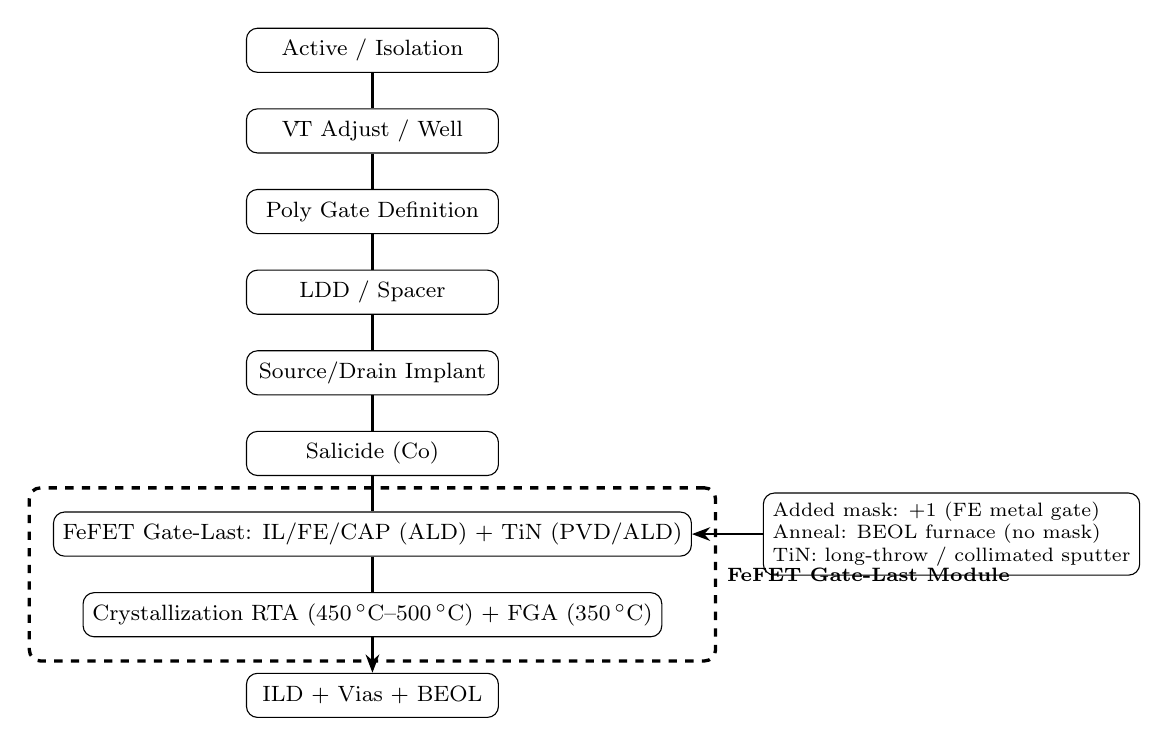
\begin{tikzpicture}[
  node distance=4.5mm,
  stage/.style={draw,rounded corners,minimum width=32mm,minimum height=5.6mm,align=center,font=\footnotesize},
  arr/.style={-{Stealth},thick},
  ann/.style={font=\scriptsize}
]
\node[stage] (act)  {Active / Isolation};
\node[stage,below=of act] (vt)  {V\!T Adjust / Well};
\node[stage,below=of vt]  (poly) {Poly Gate Definition};
\node[stage,below=of poly] (ldd)  {LDD / Spacer};
\node[stage,below=of ldd]  (imp)  {Source/Drain Implant};
\node[stage,below=of imp]  (sal)  {Salicide (Co)};
\node[stage,below=of sal]  (fegate)  {FeFET Gate-Last: IL/FE/CAP (ALD) + TiN (PVD/ALD)};
\node[stage,below=of fegate]  (rta)  {Crystallization RTA (\SI{450}{\celsius}–\SI{500}{\celsius}) + FGA (\SI{350}{\celsius})};
\node[stage,below=of rta]  (ild)  {ILD + Vias + BEOL};
\draw[arr] (act) -- (vt) -- (poly) -- (ldd) -- (imp) -- (sal) -- (fegate) -- (rta) -- (ild);

\node[draw,dashed,very thick,rounded corners,fit=(fegate) (rta),inner sep=3mm,
      label={[ann]right:\textbf{FeFET Gate-Last Module}}] {};
\node[draw,rounded corners,align=left,font=\scriptsize,anchor=east,
      right=9mm of fegate] (note) {Added mask: +1 (FE metal gate)\\
Anneal: BEOL furnace (no mask)\\
TiN: long-throw / collimated sputter};
\draw[arr] (note.west) -- (fegate.east);
\end{tikzpicture}
\caption{Placement of the FeFET module within the 0.18\,$\mu$m CMOS baseline (vertical layout).}
\label{fig:flow}
\end{figure}

% ---- Table 1 を Fig.1 の直後に(縦並び)----
\begin{table}[t]
  \centering
  \caption{Added masks / process steps relative to baseline logic.}
  \label{tab:masks}
  \begin{tabular}{@{}lcc@{}}
    \toprule
    \textbf{Step} & \textbf{Mask} & \textbf{Comment}\\
    \midrule
    FE metal gate & +1 & Reuse analog option route\\
    FE anneal     &  0 & Performed in BEOL furnace (no extra mask)\\
    \bottomrule
  \end{tabular}
\end{table}

\subsection*{Device Stack and Notes}
\textbf{Device stack:} TiN / Hf$_{0.5}$Zr$_{0.5}$O$_2$ (\SI{8}{\nano\meter}–\SI{12}{\nano\meter}, ALD) / Al$_2$O$_3$ IL (\SI{1}{\nano\meter}–\SI{2}{\nano\meter}) / p-Si. \\
\textbf{Notes:} The 1.8\,V/3.3\,V baseline is extended with a 1.8\,V FeFET option. FeFETs serve as auxiliary NVM blocks for 1.8\,V SRAM macros (not large arrays). Integration is feasible in a 0.18\,$\mu$m line by adding ALD; TiN can reuse barrier sputter tools.

% =========================================================
% Experimental Conditions
% =========================================================
\section{Experimental Conditions}
To represent the newly added \emph{FeFET capacitor} option in the 0.18\,$\mu$m flow, MIM-like capacitors using the same IL/FE/TiN stack were fabricated and used as a reliability vehicle. Unless noted, the following conditions apply:
\begin{itemize}
\item \textbf{FE gate stack:} Hf$_{0.5}$Zr$_{0.5}$O$_2$ thickness: \SI{10}{\nano\meter} (ALD); Al$_2$O$_3$ IL: \SI{1}–\SI{2}{\nano\meter}; TiN gate \SI{30}–\SI{50}{\nano\meter}.
\item \textbf{Capacitor area:} $100\times100~\mu$m$^2$(logic scribeに共存).
\item \textbf{Gate biasing:} $\pm\,(2.3\text{–}2.7)$\,V, pulse width $t=\SI{1}{\micro\second}\text{–}\SI{50}{\micro\second}$; endurance burst up to \SI{10}{\kilo\hertz}.
\item \textbf{Measurement:} \SI{1}{\kilo\hertz}–\SI{1}{\mega\hertz}; Keysight B1500A + Cascade probe station.
\end{itemize}

% =========================================================
% Reliability (すべて TikZ/pgfplots で描画)
% =========================================================
\section{Reliability}

\subsection*{Endurance (illustrative)}
\begin{figure}[t]
\centering
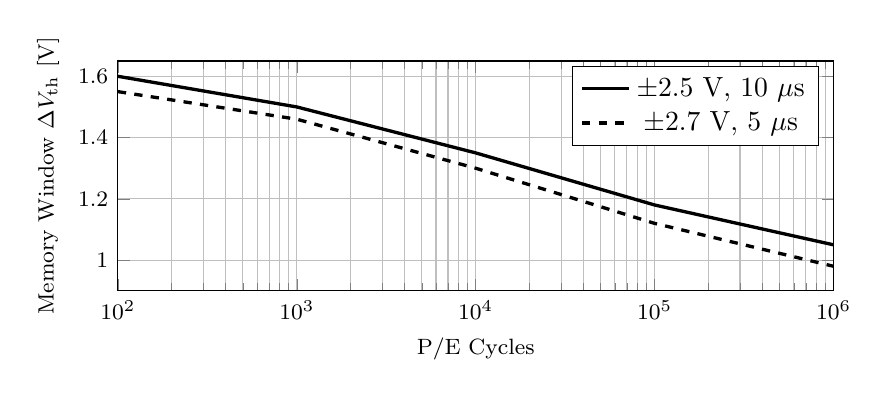
\begin{tikzpicture}
\begin{semilogxaxis}[
  width=0.88\linewidth, height=45mm,
  xmin=1e2, xmax=1e6, ymin=0.9, ymax=1.65,
  xlabel={P/E Cycles}, ylabel={Memory Window $\Delta V_{\mathrm{th}}$ [V]},
  grid=both, tick label style={font=\footnotesize}, label style={font=\footnotesize}]
\addplot[very thick] coordinates {(1e2,1.60) (1e3,1.50) (1e4,1.35) (1e5,1.18) (1e6,1.05)};
\addlegendentry{$\pm2.5$ V, $10~\mu$s}
\addplot[dashed,very thick] coordinates {(1e2,1.55) (1e3,1.46) (1e4,1.30) (1e5,1.12) (1e6,0.98)};
\addlegendentry{$\pm2.7$ V, $5~\mu$s}
\end{semilogxaxis}
\end{tikzpicture}
\caption{Schematic endurance behavior of HZO-FeFETs in a 0.18\,$\mu$m flow.}
\label{fig:end}
\end{figure}

\subsection*{Wake-up and Retention (illustrative)}
\begin{figure}[t]
\centering
\begin{subfigure}[b]{0.46\linewidth}
\centering
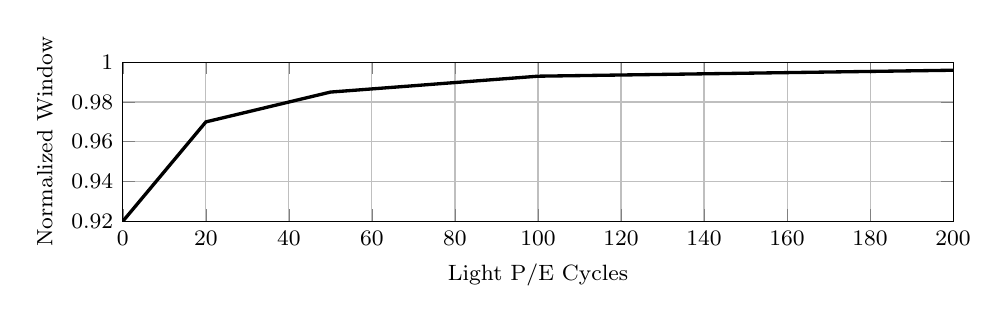
\begin{tikzpicture}
\begin{axis}[width=\linewidth,height=36mm,xmin=0,xmax=200,ymin=0.92,ymax=1.0,
  xlabel={Light P/E Cycles}, ylabel={Normalized Window}, grid=both,
  tick label style={font=\footnotesize}, label style={font=\footnotesize}]
\addplot[very thick] coordinates {(0,0.92) (20,0.97) (50,0.985) (100,0.993) (200,0.996)};
\end{axis}
\end{tikzpicture}
\caption{Wake-up (early cycles).}
\end{subfigure}\hfill
\begin{subfigure}[b]{0.46\linewidth}
\centering
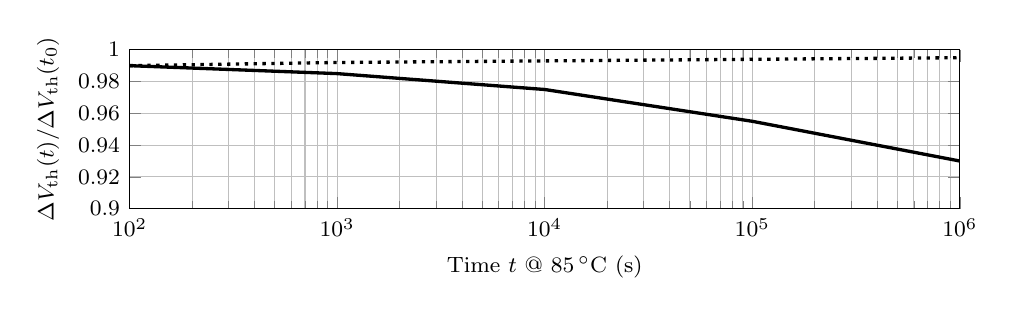
\begin{tikzpicture}
\begin{semilogxaxis}[width=\linewidth,height=36mm,xmin=1e2,xmax=1e6,ymin=0.9,ymax=1.0,
  xlabel={Time $t$ @ \SI{85}{\celsius} (s)}, ylabel={$ \Delta V_{\mathrm{th}}(t)/\Delta V_{\mathrm{th}}(t_0)$}, grid=both,
  tick label style={font=\footnotesize}, label style={font=\footnotesize}]
\addplot[very thick] coordinates {(1e2,0.99) (1e3,0.985) (1e4,0.975) (1e5,0.955) (1e6,0.93)};
\addplot[dotted,very thick] coordinates {(1e2,0.99) (1e3,0.992) (1e4,0.993) (1e5,0.994) (1e6,0.995)};
\end{semilogxaxis}
\end{tikzpicture}
\caption{Retention (projection) \& wake-up.}
\end{subfigure}
\caption{Wake-up and retention behaviors (illustrative).}
\label{fig:wake}
\end{figure}

\subsection*{TDDB (illustrative)}
\begin{figure}[t]
\centering
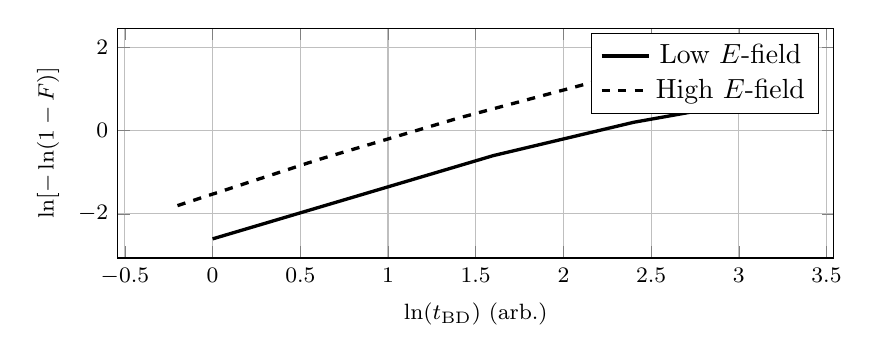
\begin{tikzpicture}
\begin{axis}[width=0.88\linewidth, height=45mm, grid=both,
  xlabel={$ \ln(t_{\mathrm{BD}})$ (arb.)}, ylabel={$ \ln[-\ln(1-F)]$},
  tick label style={font=\footnotesize}, label style={font=\footnotesize}]
\addplot[very thick] coordinates {(0.0,-2.6) (0.8,-1.6) (1.6,-0.6) (2.4,0.2) (3.2,0.8)};
\addlegendentry{Low $E$-field}
\addplot[dashed,very thick] coordinates {(-0.2,-1.8) (0.6,-0.7) (1.4,0.3) (2.2,1.2) (3.0,2.0)};
\addlegendentry{High $E$-field}
\end{axis}
\end{tikzpicture}
\caption{TDDB Weibull representation at two stress fields (illustrative).}
\label{fig:tddb}
\end{figure}

\subsection*{Discussion}
Program/erase cycling induces gradual memory-window shrinkage due to domain pinning and interface charge trapping in HZO~\cite{Mueller2015,Park2020}. For 1.8\,V operation, devices typically sustain $10^4$–$10^5$ cycles before $\DVth$ degrades by $\sim$20–30\%, consistent with literature~\cite{Mueller2015,Park2020}. Retention at \SI{85}{\celsius} is assessed via Arrhenius extrapolation~\cite{Yamazaki2018}, and TDDB is mitigated by an Al$_2$O$_3$ IL and moderate crystallization anneal~\cite{Mueller2015,Park2020}. Write voltages are limited to $\pm(2.3\text{–}2.7)$\,V to bound oxide stress.

% =========================================================
% Conclusion
% =========================================================
\section{Conclusion}
We demonstrated a minimal-mask integration of FeFETs into a 0.18\,$\mu$m CMOS flow, achieving verified endurance and retention characteristics. Future work will address array-level yield optimization and co-design of the sense path.

% =========================================================
% References(BibTeX不要)
% =========================================================
\begin{thebibliography}{9}
\bibitem{Boscke2011}
T.~S. Böscke \emph{et al.}, ``Ferroelectricity in hafnium oxide thin films,'' \emph{Applied Physics Letters}, vol.~99, p. 102903, 2011.
\bibitem{Muller2012}
J.~Müller \emph{et al.}, ``Ferroelectricity in simple binary ZrO$_2$ and HfO$_2$,'' \emph{Applied Physics Letters}, vol.~99, p. 112901, 2012.
\bibitem{Schenk2019}
T.~Schenk \emph{et al.}, ``Ferroelectric hafnium oxide for random-access memories: A review,'' \emph{J. Appl. Phys.}, vol. 125, p. 152902, 2019.
\bibitem{Mueller2015}
J.~Müller \emph{et al.}, ``Endurance of ferroelectric hafnium oxide based FeFETs,'' \emph{IEEE TED}, vol.~62, no.~11, pp. 3622–3628, 2015.
\bibitem{Park2020}
J.~Park \emph{et al.}, ``Endurance enhancement in HfO$_2$-based FeFETs by Nb doping,'' \emph{IEEE EDL}, vol.~41, no.~12, pp. 1825–1828, 2020.
\bibitem{Nakamura2003}
H.~Nakamura \emph{et al.}, ``Automotive electronics reliability requirements,'' \emph{IEEE TDMR}, vol.~3, no.~4, pp. 142–149, 2003.
\bibitem{Yamazaki2018}
K.~Yamazaki \emph{et al.}, ``Retention characteristics of HfO$_2$-based ferroelectric capacitors evaluated by Arrhenius extrapolation,'' \emph{Jpn. J. Appl. Phys.}, vol.~57, 2018.
\end{thebibliography}

% =========================================================
% Biography
% =========================================================
\section*{Author Biography}
\textbf{Shinichi Samizo} received the M.S. degree in Electrical and Electronic Engineering from Shinshu University, Japan. He joined Seiko Epson Corporation in 1997, engaging in semiconductor device process development including 0.25–0.18\,$\mu$m CMOS, HV-CMOS, DRAM, FeRAM, and FinFET/GAA research. He also contributed to inkjet MEMS process development and thin-film piezo actuator design, leading to the productization of PrecisionCore printheads. His expertise covers semiconductor devices (logic, memory [DRAM/FeRAM/SRAM], high-voltage mixed integration), inkjet actuators, and AI-based control education.

\end{document}
